\documentclass[letterpaper,12pt]{article}
\usepackage{array}
\usepackage{threeparttable}
\usepackage{geometry}
\geometry{letterpaper,tmargin=1in,bmargin=1in,lmargin=1.25in,rmargin=1.25in}
\usepackage{fancyhdr,lastpage}
\pagestyle{fancy}
\lhead{}
\chead{}
\rhead{}
\lfoot{}
\cfoot{}
\rfoot{\footnotesize\textsl{Page \thepage\ of \pageref{LastPage}}}
\renewcommand\headrulewidth{0pt}
\renewcommand\footrulewidth{0pt}
\usepackage[format=hang,font=normalsize,labelfont=bf]{caption}
\usepackage{listings}
\usepackage{booktabs}
\lstset{frame=single,
  language=Python,
  showstringspaces=false,
  columns=flexible,
  basicstyle={\small\ttfamily},
  numbers=none,
  breaklines=true,
  breakatwhitespace=true
  tabsize=3
}
\usepackage{amsmath}
\usepackage{amssymb}
\usepackage{amsthm}
\usepackage{harvard}
\usepackage{setspace}
\usepackage{float,color}
\usepackage[pdftex]{graphicx}
\usepackage{hyperref}
\usepackage{pgfplotstable}
\hypersetup{colorlinks,linkcolor=red,urlcolor=blue}
\theoremstyle{definition}
\newtheorem{theorem}{Theorem}
\newtheorem{acknowledgement}[theorem]{Acknowledgement}
\newtheorem{algorithm}[theorem]{Algorithm}
\newtheorem{axiom}[theorem]{Axiom}
\newtheorem{case}[theorem]{Case}
\newtheorem{claim}[theorem]{Claim}
\newtheorem{conclusion}[theorem]{Conclusion}
\newtheorem{condition}[theorem]{Condition}
\newtheorem{conjecture}[theorem]{Conjecture}
\newtheorem{corollary}[theorem]{Corollary}
\newtheorem{criterion}[theorem]{Criterion}
\newtheorem{definition}[theorem]{Definition}
\newtheorem{derivation}{Derivation} % Number derivations on their own
\newtheorem{example}[theorem]{Example}
\newtheorem{exercise}[theorem]{Exercise}
\newtheorem{lemma}[theorem]{Lemma}
\newtheorem{notation}[theorem]{Notation}
\newtheorem{problem}[theorem]{Problem}
\newtheorem{proposition}{Proposition} % Number propositions on their own
\newtheorem{remark}[theorem]{Remark}
\newtheorem{solution}[theorem]{Solution}
\newtheorem{summary}[theorem]{Summary}
%\numberwithin{equation}{section}
\bibliographystyle{aer}
%\newcommand\ve{\varepsilon}
%\newcommand\boldline{\arrayrulewidth{1pt}\hline}


\begin{document}

\begin{flushleft}
  \textbf{\large{Problem Set \#[4]}} \\
  MACS 40000, Dr. Evans \\
  Fiona Fan
\end{flushleft}

\vspace{5mm}

\noindent\textbf{Problem 7.1}
\\ \textbf{Part (i).} 
\begin{align}
\frac{\partial g_{cfe}(n)}{\partial n}=n^{\frac{1}{\theta}}\\
\frac{\partial g_{elp}(n)}{\partial n}=\frac{b (\frac{n}{\tilde{l}})^\upsilon (1-(\frac{n}{\tilde{l}})^\upsilon)^{(\frac{1}{\upsilon}-1)}}{n}
\end{align}

\textbf{Part (ii).} Please see Fig \ref{Fig1}

\noindent\textbf{Problem 7.2}
\\ \textbf{Part (i).} $u'(c)$=[  1.40829679e+11   5.75433098e+10   4.59479342e+00   1.22196463e-01]
\\ \textbf{Part (ii).} $g'(n)$=[ -3.24975000e+00  -4.99750001e-01   3.60237454e-01   1.01976045e+05
1.60214791e+05] 

\begin{figure}[htb]
	\centering
	\captionsetup{width=4.0in}
	\caption{\textbf{Problem 7.1 Part (ii)}}
	\label{Fig1}
	\fbox{\resizebox{4.0in}{3.0in}{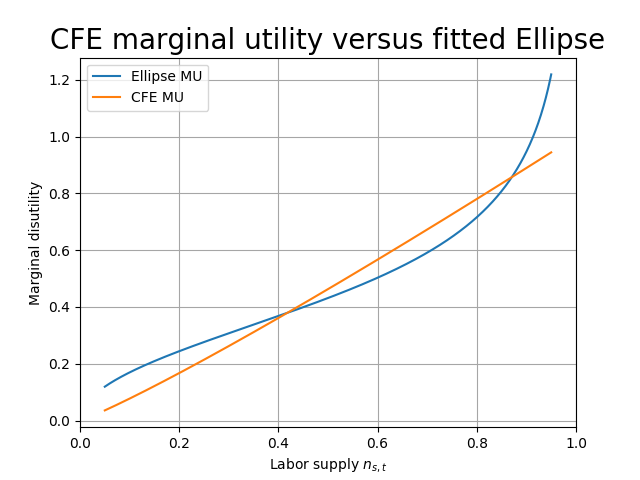
\includegraphics{fig1.png}}}
	
\end{figure}

\end{document}

